% f-pivot-wide — reshaping the stored long (time-series) data to the daily-wide
% layout the models consume. Standalone TikZ; caption lives in the chapter.
\documentclass[tikz,border=6pt]{standalone}
\usepackage{booktabs}
\usetikzlibrary{positioning, arrows.meta, fit}

\begin{document}
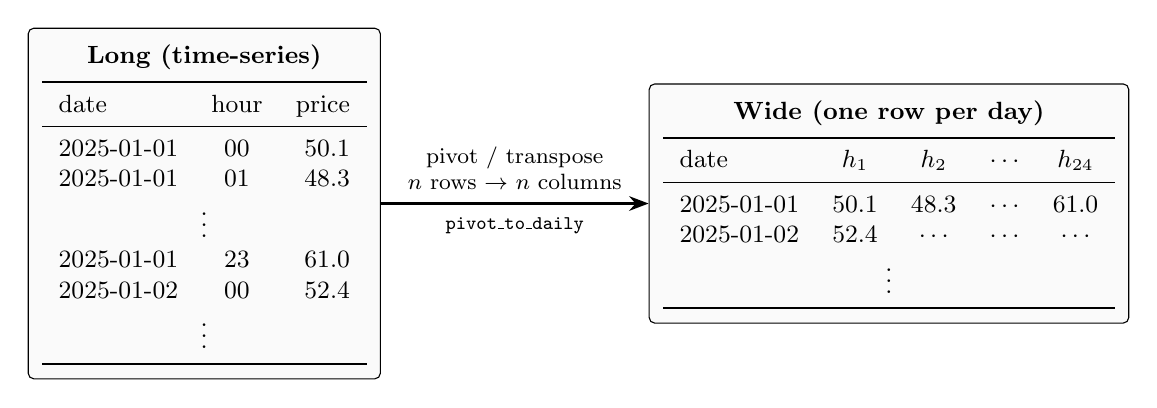
\begin{tikzpicture}[
  >={Stealth[length=7pt]},
  tbl/.style={draw, rounded corners=2pt, inner sep=5pt, fill=gray!4},
]

% --- LONG (time-series) table: one row per hour ---
\node[tbl] (long) {%
  \small
  \begin{tabular}{l c r}
    \multicolumn{3}{c}{\textbf{Long (time-series)}}\\[3pt]
    \toprule
    date & hour & price\\
    \midrule
    2025-01-01 & 00 & 50.1\\
    2025-01-01 & 01 & 48.3\\
    \multicolumn{3}{c}{$\vdots$}\\
    2025-01-01 & 23 & 61.0\\
    2025-01-02 & 00 & 52.4\\
    \multicolumn{3}{c}{$\vdots$}\\
    \bottomrule
  \end{tabular}%
};

% --- WIDE (daily) table: one row per day, the 24 hours as columns ---
\node[tbl, right=3.4cm of long] (wide) {%
  \small
  \begin{tabular}{l c c c c}
    \multicolumn{5}{c}{\textbf{Wide (one row per day)}}\\[3pt]
    \toprule
    date & $h_{1}$ & $h_{2}$ & $\cdots$ & $h_{24}$\\
    \midrule
    2025-01-01 & 50.1 & 48.3 & $\cdots$ & 61.0\\
    2025-01-02 & 52.4 & $\cdots$ & $\cdots$ & $\cdots$\\
    \multicolumn{5}{c}{$\vdots$}\\
    \bottomrule
  \end{tabular}%
};

% --- arrow: the pivot/transpose ---
\draw[->, very thick] (long.east) -- (wide.west)
  node[midway, above=1pt, align=center, font=\footnotesize]{pivot / transpose\\$n$ rows $\to$ $n$ columns}
  node[midway, below=1pt, align=center, font=\scriptsize\ttfamily]{pivot\_to\_daily};

\end{tikzpicture}
\end{document}
